\documentclass[sigconf,nonacm]{acmart}

\settopmatter{printacmref=false}
\setcopyright{none}
\renewcommand\footnotetextcopyrightpermission[1]{}
\acmConference[Security Insider Lab II]{Security Insider Lab II Mini Project}{July 2026}{University of Passau}
\acmYear{2026}
\copyrightyear{2026}

\usepackage{booktabs}
\usepackage{array}
\usepackage{float}
\usepackage{tikz}
\usetikzlibrary{arrows.meta,positioning}

\newcommand{\ResultsPath}{\texttt{results/ghazal-main-iteration6-final-score-summary-20260629.md}}
\newcommand{\MetricTriplet}[5]{%
  \fill[blue!60] (#1-.24,0) rectangle (#1-.10,#2);
  \fill[orange!75] (#1-.07,0) rectangle (#1+.07,#3);
  \fill[green!60!black] (#1+.10,0) rectangle (#1+.24,#4);
  \node[rotate=35, anchor=east, font=\scriptsize] at (#1-.20,-.035) {#5};
}
\newcommand{\CountBar}[4]{%
  \fill[green!60!black] (#1-.28,0) rectangle (#1+.28,#2);
  \fill[red!65] (#1-.28,#2) rectangle (#1+.28,#2+#3);
  \node[rotate=35, anchor=east, font=\scriptsize] at (#1-.22,-18) {#4};
}

\begin{document}

\title{HermSec-MoA: Comparing Scanner-Aided, Single-Agent, Multi-Agent, and Hybrid Repository Security Review}

\author{Seth Whenton}
\affiliation{%
  \institution{University of Passau}
  \city{Passau}
  \country{Germany}}
\email{}

\author{Ghazal Pouresfandiyar Borojeni}
\affiliation{%
  \institution{University of Passau}
  \city{Passau}
  \country{Germany}}
\email{}

\begin{abstract}
HermSec is a desktop app that scans local code repositories for security issues. The main goal is simple. A user should pick a project, press scan, and get a clear report. HermSec first checks the project type, chooses useful scanners, runs the tools, and writes a report. The app also supports model-aided review.

This paper reports completed tests on our Ghazal dataset of 20 projects and 184 labelled findings. The tested configurations were Deep assisted scan, Single Agent inspection, MoA Low, MoA High, Scanner + MoA Low, and Scanner + MoA High. These tests compare scanner-backed review, direct agent review, multi-agent review, and a hybrid scanner-agent review.

The best F1 score was Scanner + MoA High with 0.7640. Single Agent reached 0.6462 and was faster. MoA High reached 0.5455, MoA Low reached 0.5433, Scanner + MoA Low reached 0.5333, and Deep assisted reached 0.4381. The result shows that the hybrid mode gave the strongest balance. The current HermSec software uses candidate-first tasks, bounded file tools, evidence checks, sanitizer-aware filtering, and efficient non-US models to make these modes more reliable.
\end{abstract}

\keywords{static analysis, software security, repository scanning, multi-agent systems, vulnerability detection, code review}

\maketitle

\section{Introduction}
Developers need security feedback while they work. Static application security testing tools help because they can check source code without running the program \cite{chess2004static,livshits2005finding}. These tools are useful, but they can also miss bugs or report too many false alarms \cite{zitser2004testing}.

HermSec was built as a simple desktop security scanner for local projects. The user selects a folder and asks HermSec to scan it. HermSec inspects the repository, detects languages and project files, chooses the scanners that fit the project, runs the scan, and writes a report. This matters because a JavaScript project, Java project, Python project, Rust project, and PHP project do not need the same scanner set.

The project also studies model-aided security review. We wanted to know if agent inspection can improve the normal scanner workflow. We also wanted to test if a mixture of agents can do better than a single model. Finally, we tested a hybrid mode where scanners and MoA agents run separately, then a judge and aggregator merge the findings.

The research question is:

\begin{quote}
Can HermSec improve repository security review by combining static scanners, single-agent inspection, MoA inspection, and Scanner + MoA aggregation while using efficient low-cost models?
\end{quote}

This paper explains the current HermSec product, the scan modes, the dataset, the results, and the next work needed.

\section{HermSec Product Overview}
HermSec is not only a command line test tool. It is a desktop app with a chat-style workflow. The app has project selection, scan mode selection, live progress cards, scanner settings, model provider settings, Doctor checks, automation settings, and report links.

The most important product idea is the scan flow. HermSec first inspects the project. It checks files, languages, package manifests, lockfiles, and configuration files. It then chooses the scanners that match the project. For example, a Node.js project can use JavaScript rules, dependency checks, and secret scanning. A Python project can use Python rules, Bandit, pip-audit style checks, and dependency intelligence. A Java project can use Java rules and Java taint heuristics. This adaptive choice helps avoid installing or running every scanner for every project.

HermSec currently supports built-in heuristics and external scanners such as Semgrep, Gitleaks, Trivy, Bandit, OSV-Scanner, and Checkov \cite{semgrep,gitleaks,trivy,bandit,osvscanner,checkov}. The app can show which scanners are installed, missing, enabled, and useful for the current project.

Figure~\ref{fig:app-scan} shows the scan workflow. The user chooses a scan mode, then HermSec keeps the progress card in the chat and writes the report when the scan finishes.

\begin{figure*}[!htbp]
  \centering
  
\includegraphics[width=.49\textwidth]{figures/hermsec_scan_choice_progress.png}\hfill
  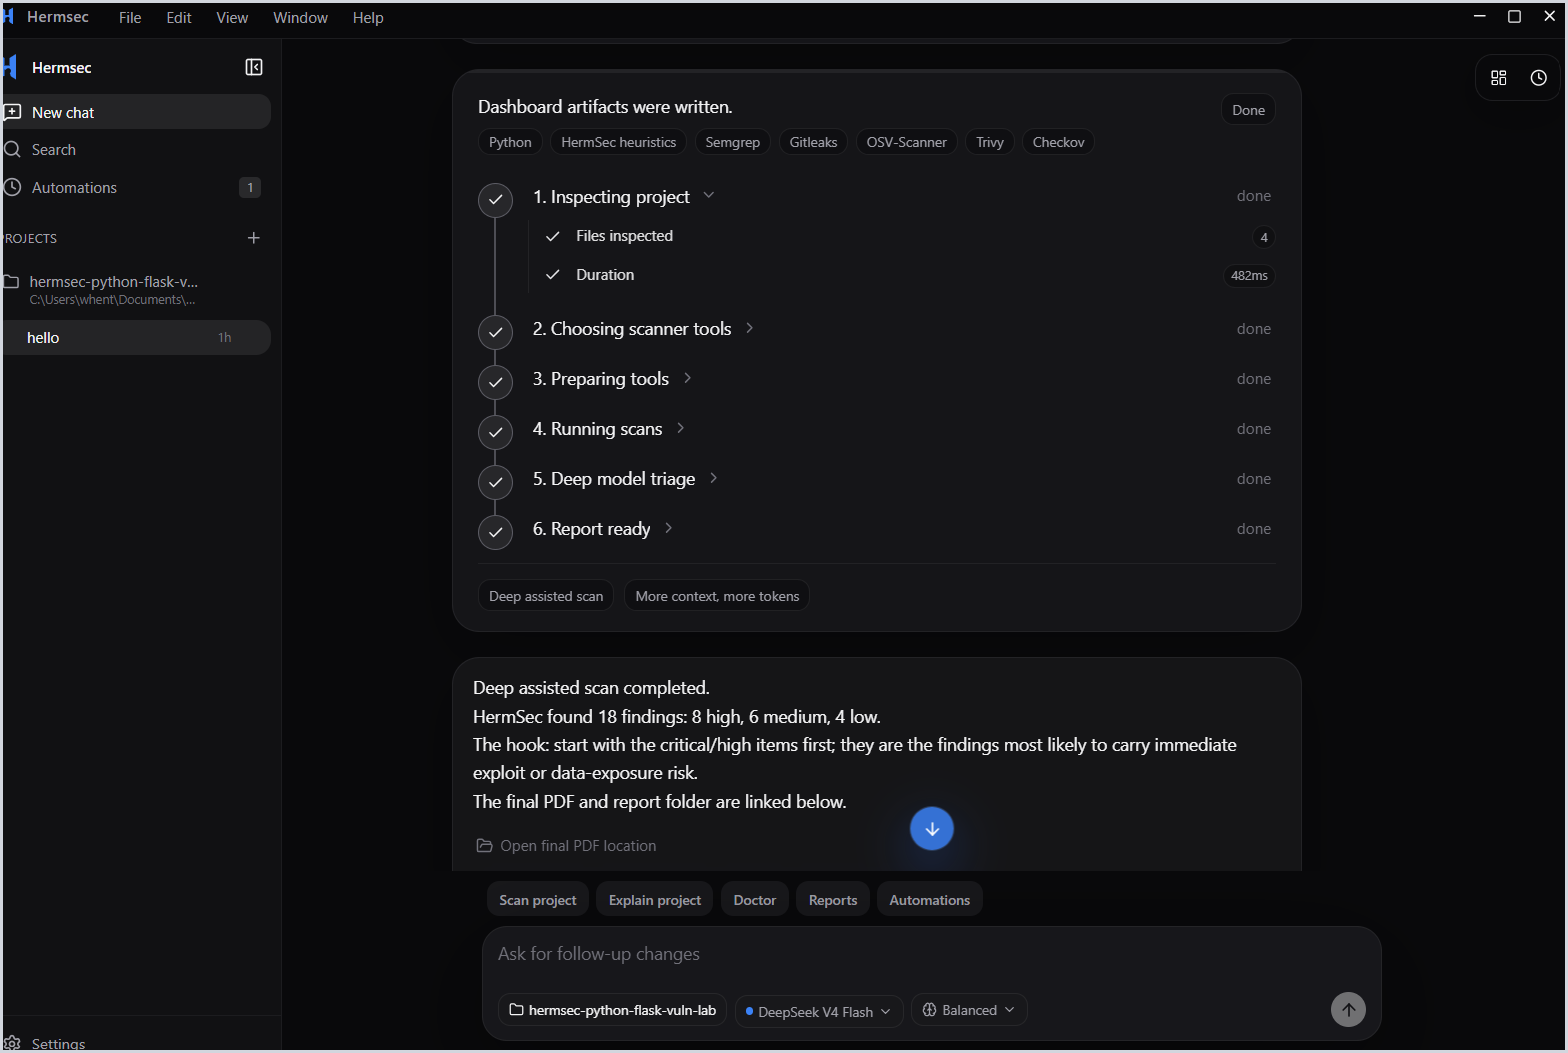
\includegraphics[width=.49\textwidth]{figures/hermsec_scan_completed_summary.png}
  \caption{HermSec scan workflow. The app asks the user to choose a mode, shows progress, and then shows a short report summary.}
  \Description{Two screenshots of HermSec. The first shows scan mode selection and a live progress card. The second shows a completed scan and final report text.}
  \label{fig:app-scan}
\end{figure*}

Figure~\ref{fig:app-settings} shows the settings pages for agent and provider setup. Figure~\ref{fig:scanner-settings} shows scanner management.

\begin{figure*}[!htbp]
  \centering
  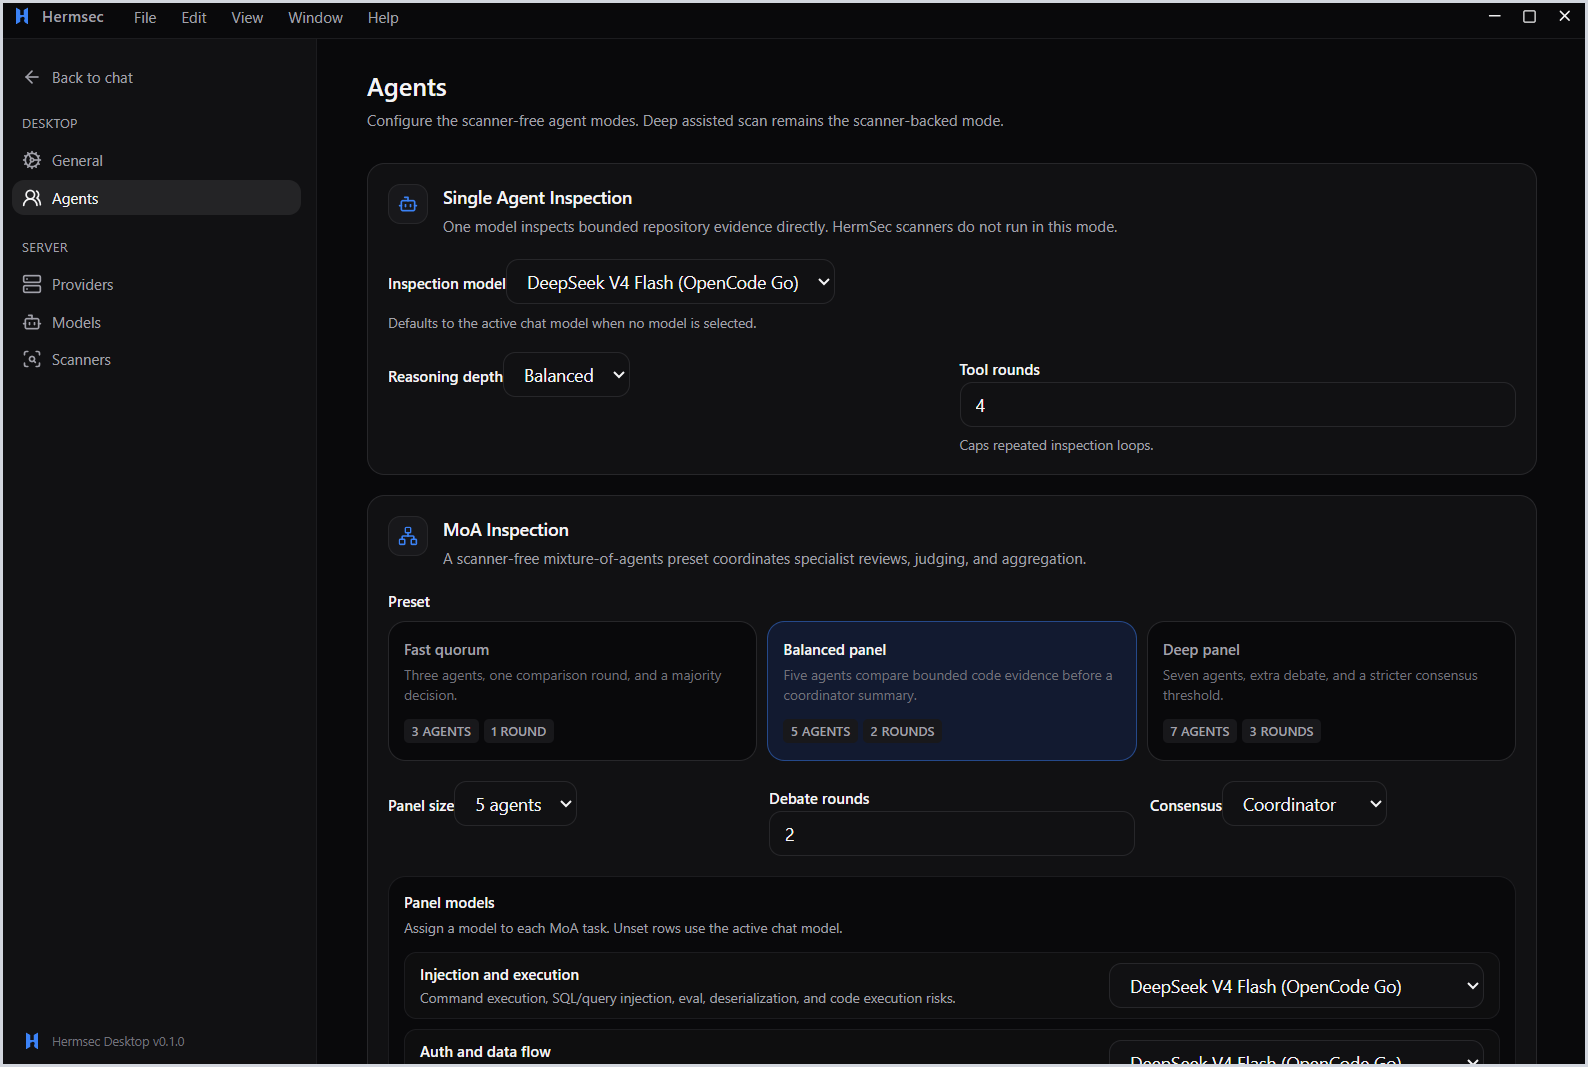
\includegraphics[width=.49\textwidth]{figures/hermsec_agents_settings_full.png}\hfill
  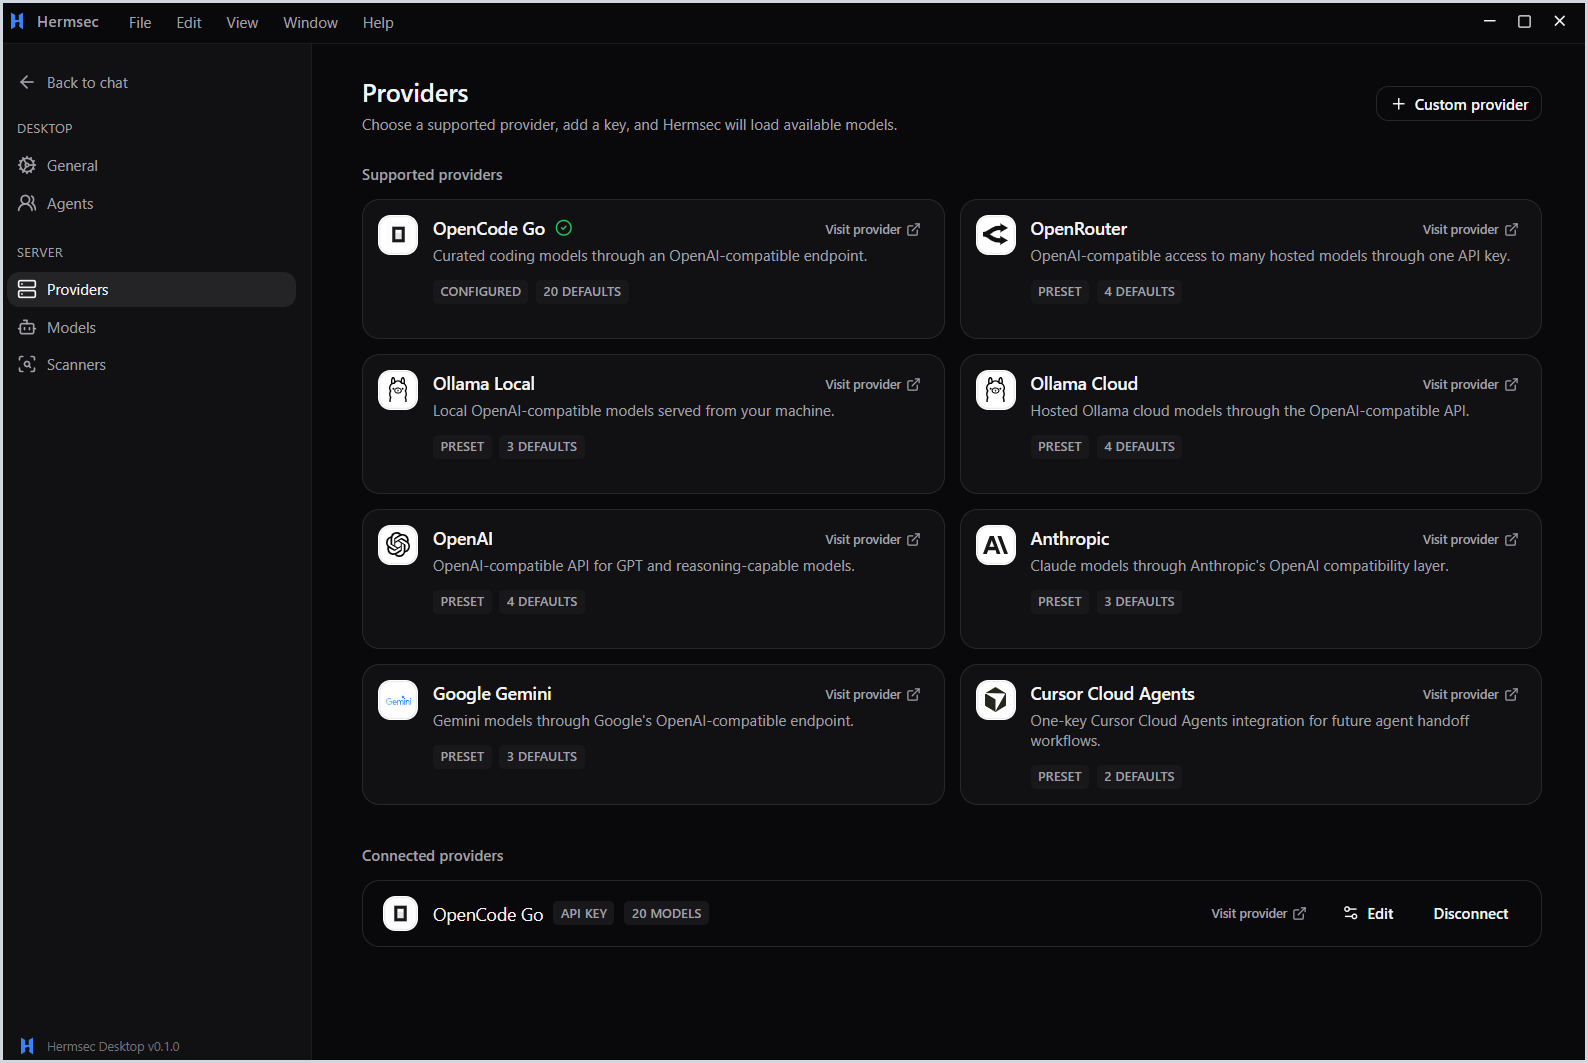
\includegraphics[width=.49\textwidth]{figures/hermsec_providers_settings.png}
  \caption{HermSec settings. Left: Single Agent and MoA settings. Right: model provider setup.}
  \Description{Two screenshots of the settings screens. One shows agent settings and the other shows provider cards.}
  \label{fig:app-settings}
\end{figure*}

\begin{figure*}[!htbp]
  \centering
  
\includegraphics[width=.72\textwidth]{figures/hermsec_scanners_settings.png}
  \caption{Scanner settings show installed, missing, enabled, and project-relevant tools.}
  \Description{A screenshot of scanner settings showing rows for scanners and install states.}
  \label{fig:scanner-settings}
\end{figure*}

\section{Related Work}
Static analysis has been used for many years to detect security problems before code runs \cite{chess2004static,livshits2005finding}. It is still important because it is fast and can run in development. However, static tools need careful rules and testing. Benchmarks and labelled examples help show where a tool is strong or weak \cite{zitser2004testing}.

Modern scanners often focus on different areas. Semgrep is useful for rule-based source scanning. Gitleaks is used for secrets. Trivy and OSV-Scanner support dependency and advisory checks. Bandit is used for Python security linting \cite{semgrep,gitleaks,trivy,bandit,osvscanner}. HermSec uses this multi-tool idea and normalizes findings into one report.

Large language models can help explain code, but they can also make false claims \cite{pearce2022asleep}. Agent patterns such as ReAct show how a model can use tools step by step \cite{yao2023react}. Multi-agent debate and mixture-of-agents work also show that several model answers can improve some tasks \cite{du2023debate,wang2024moa}. HermSec uses a similar idea for code review. The MoA settings were also inspired by configurable agent panels in Hermes Agent \cite{nous2026hermesagent}.

\section{Current HermSec Techniques}
HermSec has four visible scan modes. MoA and Scanner + MoA have Low and High panel settings in the app. This paper records the latest Ghazal results for Deep assisted, Single Agent, MoA Low, MoA High, Scanner + MoA Low, and Scanner + MoA High.

\subsection{Deep Assisted Scan}
Deep assisted scan is scanner-backed. HermSec inspects the repository, chooses scanner tools, prepares them, runs them, and normalizes the findings. A model then explains scanner-backed evidence. This mode is closest to the original product idea. It gives broad tool coverage and then uses a model for summary and explanation. The current CLI also chunks model explanation work and uses watchdogs so the model step cannot block the scan forever.

\subsection{Single Agent Inspection}
Single Agent inspection does not run scanners. HermSec first creates focused investigation tasks from deterministic candidate discovery. These candidates cover source-to-sink patterns such as SQL injection, command execution, path traversal, XSS, hardcoded secrets, redirects, dependency risk, and configuration risk. The model receives bounded repository evidence using safe read-only tools: list files, search code, and read snippets. The model cannot execute shell commands, install packages, or read outside the selected repository. After the model proposes findings, HermSec checks that files and snippets really exist before adding findings to the report.

\subsection{MoA Inspection}
MoA inspection uses several specialist agents. The Low panel uses three specialists: injection and execution, auth and data flow, and secrets and config. The High panel uses five specialists by adding database and storage, and config and IaC. A false-positive judge checks the candidate findings. An aggregator then writes the final accepted findings.

This design improves simple broad prompting because agents do not just receive "inspect this repo". They receive focused tasks, such as checking an injection candidate, a hardcoded secret candidate, or a sanitizer claim. This should reduce token waste because each agent reads selected evidence instead of reading the whole project. The judge rejects unsupported model claims instead of keeping them for human review.

\subsection{Scanner + MoA Inspection}
Scanner + MoA is the hybrid mode. Scanners run normally and produce scanner findings. MoA agents also inspect the project separately. The judge receives both scanner candidates and agent candidates. The aggregator deduplicates and writes the final findings.

This mode tries to get the coverage advantage of scanners and the reasoning advantage of agents. It is also the most expensive mode because it runs both scanner and agent work. The current design adds final evidence validation so unsupported model claims are rejected. The latest CLI also adds sanitizer-aware filtering for safe patterns such as prepared SQL statements, HTML escaping, canonical path checks, \texttt{basename}, and \texttt{filepath.Clean}. This reduced clean-project false positives in the final Scanner + MoA High run.

\subsection{Efficient Model Routing}
The experiment used OpenCode Go as the provider route \cite{opencodego}. Deep assisted and Single Agent used \texttt{deepseek-v4-flash}. MoA and Scanner + MoA used \texttt{deepseek-v4-flash}, \texttt{mimo-v2.5}, \texttt{deepseek-v4-pro}, and \texttt{minimax-m3}. We avoided US flagship models in the experiment table.

This model choice was made for cost and speed reasons. DeepSeek documents context caching and lower cached-token pricing \cite{deepseekcache,deepseekpricing}. MiMo V2.5 is described as an agent-capable model family with inference optimization work \cite{xiaomimimo25,xiaomimimo25inference}. MiniMax-M3 is presented as a coding and agentic model \cite{minimaxm3}. We did not measure exact money cost in this run, so cost claims are design claims, not final cost measurements.

\section{Harness Flow}
Every HermSec scan starts with repository inspection. Then the selected mode runs. After the mode finishes, HermSec validates evidence, deduplicates findings, normalizes them, and writes HTML, JSON, and PDF-ready report artifacts.

\begin{figure*}[!htbp]
  \centering
  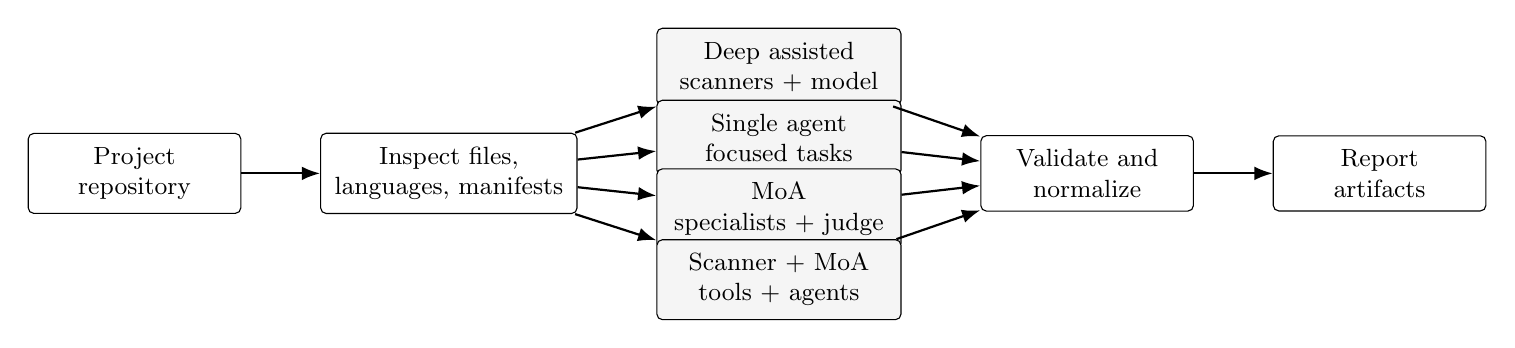
\begin{tikzpicture}[
    font=\small,
    box/.style={draw, rounded corners=2pt, align=center, inner sep=5pt, minimum width=2.7cm, minimum height=.7cm},
    mode/.style={draw, rounded corners=2pt, align=center, inner sep=5pt, minimum width=3.1cm, minimum height=.7cm, fill=gray!8},
    arrow/.style={-Latex, thick}
  ]
    \node[box] (repo) {Project\\repository};
    \node[box, right=1.0cm of repo] (inspect) {Inspect files,\\languages, manifests};
    \node[mode, right=1.0cm of inspect, yshift=1.35cm] (deep) {Deep assisted\\scanners + model};
    \node[mode, right=1.0cm of inspect, yshift=.45cm] (single) {Single agent\\focused tasks};
    \node[mode, right=1.0cm of inspect, yshift=-.45cm] (moa) {MoA\\specialists + judge};
    \node[mode, right=1.0cm of inspect, yshift=-1.35cm] (hybrid) {Scanner + MoA\\tools + agents};
    \node[box, right=1.0cm of single, yshift=-.45cm] (validate) {Validate and\\normalize};
    \node[box, right=1.0cm of validate] (report) {Report\\artifacts};

    \draw[arrow] (repo) -- (inspect);
    \draw[arrow] (inspect) -- (deep);
    \draw[arrow] (inspect) -- (single);
    \draw[arrow] (inspect) -- (moa);
    \draw[arrow] (inspect) -- (hybrid);
    \draw[arrow] (deep) -- (validate);
    \draw[arrow] (single) -- (validate);
    \draw[arrow] (moa) -- (validate);
    \draw[arrow] (hybrid) -- (validate);
    \draw[arrow] (validate) -- (report);
  \end{tikzpicture}
  \caption{Current HermSec harness flow. The selected mode changes how findings are created, but all final findings pass through validation and reporting.}
  \Description{A flow diagram from project repository to inspection, four scan modes, validation, and final reports.}
  \label{fig:harness-flow}
\end{figure*}

\section{Method}
\subsection{Dataset}
We tested HermSec on our dataset of 20 local projects. The dataset contains 184 labelled findings. It includes vulnerable and clean projects across JavaScript, TypeScript, Python, Java, PHP, Ruby, Go, Rust, C/C++, C\#, Docker, and GitHub Actions style configuration. The findings cover injection, command execution, secrets, authentication, dependency risk, database risk, API risk, crypto issues, and configuration problems. CWE labels were used where possible \cite{mitrecwe}. The risk types also match common web security issues described by OWASP \cite{owasptop10}.

\subsection{Modes Tested}
The final metric table uses the completed full-dataset runs. The tested configurations were:

\begin{itemize}
  \item Deep assisted scan with \texttt{deepseek-v4-flash}.
  \item Single Agent with \texttt{deepseek-v4-flash}.
  \item MoA Low with three specialists, a judge, and an aggregator.
  \item MoA High with five specialists, a judge, and an aggregator.
  \item Scanner + MoA Low with scanners and the low MoA panel.
  \item Scanner + MoA High with scanners and the high MoA panel.
\end{itemize}

The MoA and Scanner + MoA model pool was \texttt{deepseek-v4-flash}, \texttt{mimo-v2.5}, \texttt{deepseek-v4-pro}, and \texttt{minimax-m3}. All model calls used OpenCode Go. Scanner + MoA Low completed 17 of 20 runs, so it is included as a secondary row. Scanner + MoA High completed all 20 runs and is the main hybrid result.

\subsection{Metrics}
We used true positives, false positives, false negatives, precision, recall, and F1. Precision means the share of reported findings that were correct. Recall means the share of labelled findings that were found. F1 is the balance between precision and recall.

Each main configuration was run against the 20 projects. Scanner + MoA Low completed 17 successful runs; the other rows completed 20 successful runs. The raw comparison note is saved at \ResultsPath.

\section{Results}
Table~\ref{tab:main-results} gives the main result. Figure~\ref{fig:metric-chart} shows precision, recall, and F1. Figure~\ref{fig:count-chart} shows the true-positive and false-positive output count.

\begin{table*}[!htbp]
  \centering
  \caption{Main results from completed full runs on the Ghazal dataset.}
  \label{tab:main-results}
  \begin{tabular}{lrrrrrrrrr}
    \toprule
    Mode & Runs & OK & TP & FP & FN & Precision & Recall & F1 & Time (s) \\
    \midrule
    Deep assisted & 20 & 20 & 85 & 119 & 99 & 0.4167 & 0.4620 & 0.4381 & 715 \\
    Single Agent & 20 & 20 & 126 & 80 & 58 & 0.6117 & 0.6848 & 0.6462 & 269 \\
    MoA Low & 20 & 20 & 91 & 60 & 93 & 0.6026 & 0.4946 & 0.5433 & 1178 \\
    MoA High & 20 & 20 & 84 & 40 & 100 & 0.6774 & 0.4565 & 0.5455 & 1560 \\
    Scanner + MoA Low & 20 & 17 & 88 & 58 & 96 & 0.6027 & 0.4783 & 0.5333 & 4416 \\
    Scanner + MoA High & 20 & 20 & 157 & 70 & 27 & 0.6916 & 0.8533 & 0.7640 & 2321 \\
    \bottomrule
  \end{tabular}
\end{table*}

\begin{figure*}[!htbp]
  \centering
  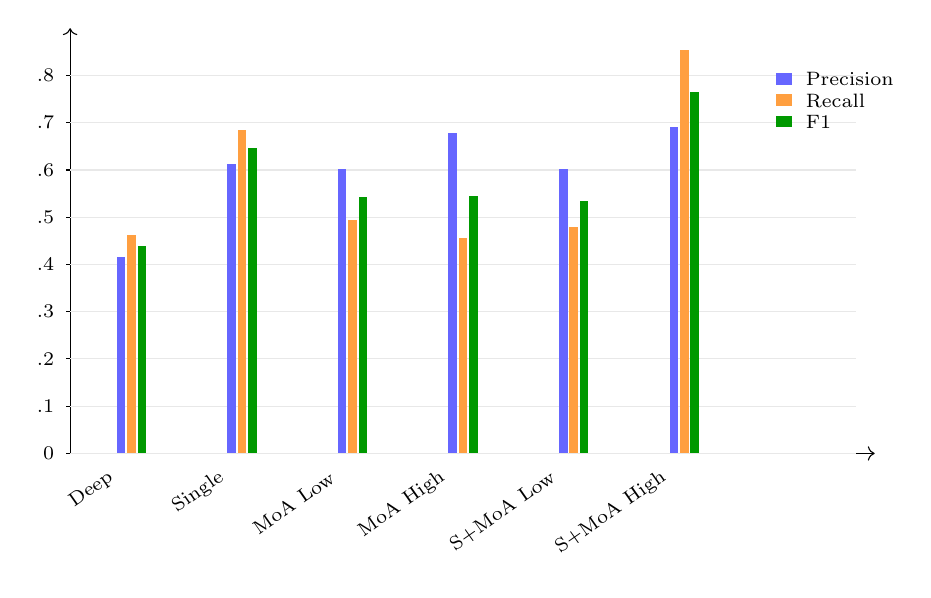
\begin{tikzpicture}[x=0.78cm,y=6.0cm,font=\scriptsize]
    \draw[->] (0,0) -- (13.1,0);
    \draw[->] (0,0) -- (0,.9);
    \foreach \y/\label in {0/0,.1/.1,.2/.2,.3/.3,.4/.4,.5/.5,.6/.6,.7/.7,.8/.8} {
      \draw (-.06,\y) -- (.06,\y);
      \node[anchor=east] at (-.1,\y) {\label};
      \draw[gray!18] (0,\y) -- (12.8,\y);
    }
    \MetricTriplet{1}{0.4167}{0.4620}{0.4381}{Deep}
    \MetricTriplet{2.8}{0.6117}{0.6848}{0.6462}{Single}
    \MetricTriplet{4.6}{0.6026}{0.4946}{0.5433}{MoA Low}
    \MetricTriplet{6.4}{0.6774}{0.4565}{0.5455}{MoA High}
    \MetricTriplet{8.2}{0.6027}{0.4783}{0.5333}{S+MoA Low}
    \MetricTriplet{10.0}{0.6916}{0.8533}{0.7640}{S+MoA High}
    \fill[blue!60] (11.5,.78) rectangle (11.75,.805);
    \node[anchor=west] at (11.82,.792) {Precision};
    \fill[orange!75] (11.5,.735) rectangle (11.75,.760);
    \node[anchor=west] at (11.82,.747) {Recall};
    \fill[green!60!black] (11.5,.690) rectangle (11.75,.715);
    \node[anchor=west] at (11.82,.702) {F1};
  \end{tikzpicture}
  \caption{Precision, recall, and F1 for the completed full Ghazal runs. Scanner + MoA High had the best F1.}
  \Description{A grouped bar chart comparing precision, recall, and F1 for six configurations.}
  \label{fig:metric-chart}
\end{figure*}

\begin{figure*}[!htbp]
  \centering
  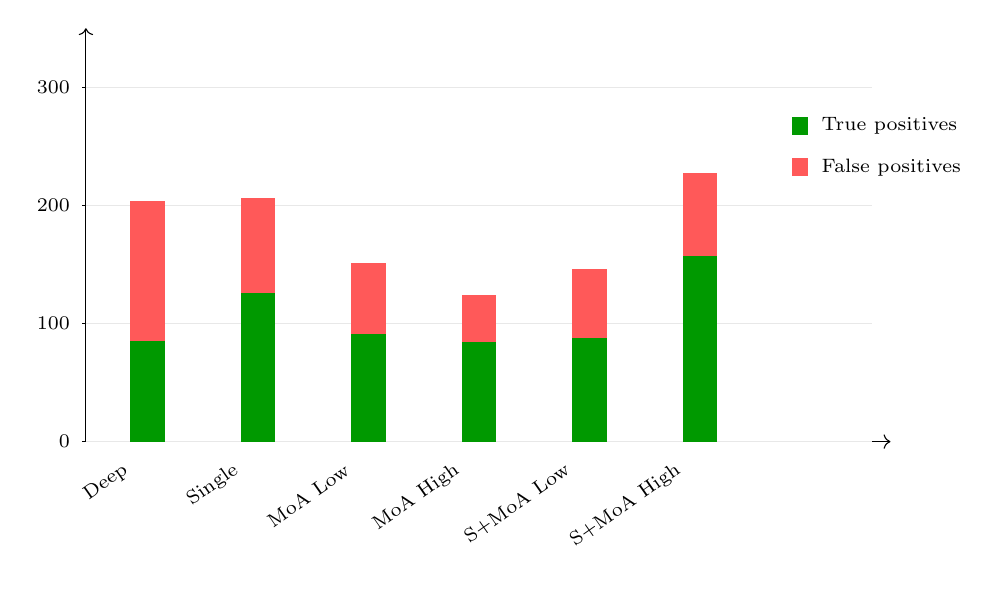
\begin{tikzpicture}[x=0.78cm,y=.015cm,font=\scriptsize]
    \draw[->] (0,0) -- (13.1,0);
    \draw[->] (0,0) -- (0,350);
    \foreach \y in {0,100,200,300} {
      \draw (-.06,\y) -- (.06,\y);
      \node[anchor=east] at (-.1,\y) {\y};
      \draw[gray!18] (0,\y) -- (12.8,\y);
    }
    \CountBar{1}{85}{119}{Deep}
    \CountBar{2.8}{126}{80}{Single}
    \CountBar{4.6}{91}{60}{MoA Low}
    \CountBar{6.4}{84}{40}{MoA High}
    \CountBar{8.2}{88}{58}{S+MoA Low}
    \CountBar{10.0}{157}{70}{S+MoA High}
    \fill[green!60!black] (11.5,260) rectangle (11.75,275);
    \node[anchor=west] at (11.82,267) {True positives};
    \fill[red!65] (11.5,225) rectangle (11.75,240);
    \node[anchor=west] at (11.82,232) {False positives};
  \end{tikzpicture}
  \caption{True-positive and false-positive counts. Scanner + MoA High found the strongest balance on this dataset.}
  \Description{A stacked bar chart showing true positives and false positives for six configurations.}
  \label{fig:count-chart}
\end{figure*}

\section{Discussion}
The result shows that the working method improved the balance between coverage and false positives. Deep assisted found 85 true positives, but it still produced 119 false positives. This is expected because it depends strongly on scanner output.

Single Agent performed well for a cheaper mode. It found 126 true positives with 80 false positives and reached an F1 score of 0.6462. This is important because it shows that focused candidate tasks and evidence checks can make one model useful without running scanners.

MoA Low and MoA High were more balanced than Deep assisted, but they did not beat Single Agent. MoA Low reached an F1 score of 0.5433. MoA High reached 0.5455. This shows that adding more agents is not automatically better. The agents need good focused tasks and good rejection rules.

Scanner + MoA High gave the best result. It found 157 true positives, had 70 false positives, and reached an F1 score of 0.7640. Scanner + MoA Low reached 0.5333, but only 17 of 20 runs completed successfully. This supports the main idea of HermSec. Scanners are useful for coverage, agents are useful for reasoning, and a judge/aggregator can merge the evidence into a stronger report.

The current candidate-first technique is useful because it avoids asking every agent to read the whole project. HermSec first builds focused tasks and then sends those tasks to the agents. The latest tuning also added sanitizer-aware filtering, so safe code such as escaped HTML, prepared SQL, canonical path checks, and cleaned paths is less likely to be reported. This reduces wasted context and helps the judge reject unsupported claims. The full run also showed a practical tradeoff. Scanner + MoA High had the best score, but Single Agent was much faster.

\section{Problems Faced}
The main problem during testing was model reliability. Some model calls returned empty content or timed out. HermSec was updated with watchdogs, shorter retries, and fallback handling so a scan would not loop forever.

Another problem was scanner noise. Scanner-backed modes can find many real issues, but they can also report too much. Clean projects were useful because they showed where scanner or hybrid modes were too noisy.

A third problem was evidence safety. Model findings can mention files or lines that do not exist. HermSec now revalidates evidence before final reporting. Unsupported model claims are rejected instead of being shown as real vulnerabilities.

A final issue was runtime. Full MoA-style runs were slower than Single Agent. This is why the product needs checkpoints, caching, and focused tasks. These features help keep the app usable even when the agent panel is larger.

\section{Threats to Validity}
The dataset is useful, but it is still limited. It has 20 local projects and 184 labelled findings. The results may change on larger real repositories. The scoring is also based on matching findings to known labels, so matching rules can affect precision and recall.

The experiment used efficient models through OpenCode Go. Different model providers, different model versions, or different temperature settings may change the result. Exact token cost was not measured, so this paper only reports runtime and finding metrics.

\section{Future Work}
Future work should make HermSec more automatic and easier to use. The long-term product goal is a much smaller app with one main scan button. The app should inspect the project, choose tools, run the right mode, and write the report with less setup.

HermSec should also support email reporting. The agent could connect to a mailbox and send scan reports after new scans. This would help scheduled security checks.

Another useful future feature is an MCP server for HermSec. This would let agents inside editing tools call the HermSec CLI directly. For example, an editor agent could ask HermSec to scan the current project, wait for the result, and open the report without the user switching tools.

Another important feature is change detection. If a project has not changed since the last scan, HermSec should know that and avoid running the same full scan again. It could compare file hashes, git commits, package lockfiles, and stored report metadata. This would save time and reduce model tokens.

The hybrid mode also needs better runtime and cost control. Scanner + MoA High gave the best result, but it took a long time. Better scanner candidate limits, stronger judge prompts, better evidence checks, caching, and cost tracking should improve it.

\section{Conclusion}
HermSec is a desktop repository security scanner with scanner-backed and agent-backed review modes. The completed Ghazal test used 20 projects and 184 labelled findings. Scanner + MoA High gave the best F1 score with 0.7640. Single Agent was the fastest strong mode with an F1 score of 0.6462.

The main lesson is simple. Scanners are useful for coverage. Agents are useful for focused reasoning and explanation. The best direction for HermSec is not only scanners or only agents. The best direction is a careful hybrid design with focused tasks, strong evidence validation, and better false-positive control.

\bibliographystyle{ACM-Reference-Format}
\bibliography{hermsec_moa_refs}

\end{document}
